\documentclass[10pt,twocolumn,letterpaper]{article}
\usepackage{times}\usepackage{graphicx}\usepackage{amsmath}\usepackage{amssymb}
\usepackage[top=1in,columnsep=0.3125in,textwidth=6.8125in,textheight=8.875in]{geometry}
\usepackage[font=small,labelsep=period]{caption}
\pagestyle{empty}
\newcommand{\bench}{OnTimeBench}
\begin{document}
\section*{4.3. Evaluation Protocol}
\paragraph{Native latency.}
During each query, physics advances by the method's own inference latency, drawn from
its latency distribution measured at batch size 1 on one GPU. All methods share
one executor, which hands over each chunk at the first control-period boundary at or after
inference completes and executes it from the command indexed to that boundary (Fig.~\ref{fig:exec}).

\begin{figure}[t]
\centering
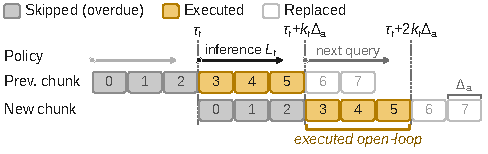
\includegraphics[width=\linewidth]{protocol_timeline.pdf}
\caption{\textbf{Native-latency executor.} Ticks: $\Delta_a=50$\,ms. Query $t$ uses the frame from $\tau_t$. At $\tau_{t+1}=\tau_t+k_t\Delta_a$, the new chunk takes over and the next query begins, with $k_t=\lceil L_t/\Delta_a\rceil$. Observation age increases while each command is held ($d_{\rm task}=0$ shown).}
\label{fig:exec}
\end{figure}

\paragraph{Settings and metrics.}
We evaluate three settings: \emph{Native}, at each method's own latency; \emph{+150\,ms},
with 150\,ms added to every method; and \emph{Paused}, with the world paused during inference. We report the task-balanced success rate (SR) and
the p95 time-to-action, the time from capturing an observation until its first command is available. The full
protocol is in the supplementary material.
A dynamic benchmark must account for the time each policy takes to compute. When the simulation advances only after the policy has returned its actions, a slow policy is scored as if it were instant. The evaluation then measures what a policy predicts, but not whether the prediction arrives in time. On a real robot, timing decides success. Observation, scene motion, and action execution share one physical clock, so the scene keeps moving for as long as each policy computes.
\end{document}
